\documentclass[fleqn]{report}

\usepackage{amsmath}
\usepackage{amssymb}
\usepackage[margin=1in]{geometry}
\usepackage{graphicx}
\graphicspath{{images/}}
\usepackage{appendix}
\usepackage{minted}

\renewcommand{\vec}[1]{\mathbf{#1}}
\DeclareMathOperator{\E}{\mathbb{E}}
\DeclareMathOperator{\I}{\mathbb{I}}

\title{Deep Learning 2018/19 - Assignment 1}

\begin{document}

\section*{Exercise 1}
In this exercise, $\sigma_n$ is used to express $\sigma \left( \vec{w}^T \vec{x}_n \right )$.

\subsection*{Exercise 1.1}
In this exercise it is required to determine the expression for the negative log likelihood for $N$ pairs of data $(x_n, c_n), c_n \in {0, 1}$. It is also reminded that the likelihood loss is $H(p_n, c_n) = - \E[\log p_n]_{c_n}$. Finally, it is known that $p_n$ is in state $1$ with probability $\sigma_n$ and since the setting is binary, it is in state $0$ with probability $1 - \sigma_n$.
\begin{equation}
    \begin{split}
        E_{lik}(\vec{w}) & = H(p_n, c_n) \\
        & = - \E[\log p_n]_{c_n} \\
        & = - \sum_{n=1}^N
        \begin{cases}
            \log \left( \sigma_n \right) & c_n = 1 \\
            \log \left(1 - \sigma_n \right) & c_n = 0
        \end{cases}
        \\ & = - \sum_{n=1}^N \I[c_n = 1] \log (\sigma_n) + \I[c_n = 0] \log (1 - \sigma_n)
    \end{split}
\end{equation}
The operator $\I[\upsilon]$ is the indicator function: it is equal to $1$ if the condition $\upsilon$ specified is true, $0$ otherwise. However, the scaled loss is required, in order to normalise it for the number of pairs.
\begin{equation}
    E_{lik}(\vec{w}) = - \frac{1}{N} \sum_{n=1}^N \I[c_n = 1] \log (\sigma_n) + \I[c_n = 0] \log (1 - \sigma_n)
\end{equation}

\subsection*{Exercise 1.2}
The question requires to determine the convexity of $E_{lik}$ with respect to $\vec{w}$. One way to do that is to determine whether the second derivative is ever negative.
\begin{equation}
    E_{lik} (\vec{w}) =
    - \frac{1}{N} \sum_{n=1}^n
    \mathbb{I}[c_n = 1] \log \sigma_n
    + \mathbb{I}[c_n = 0] \log \left ( 1 - \sigma_n \right )
\end{equation}
\begin{equation}
    \begin{split}
        \frac{\partial E}{\partial \vec{w}} & =
        - \frac{1}{N} \sum_{n=1}^n
        \mathbb{I}[c_n = 1]
        \frac{x_n \sigma_n (1 - \sigma_n)}{\sigma_n}
        - \mathbb{I}[c_n = 0]
        \frac{x_n \sigma_n (1 - \sigma_n)}{1 - \sigma_n} \\
        & = - \frac{1}{N} \sum_{n=1}^n
        \mathbb{I}[c_n = 1]
        x_n (1 - \sigma_n)
        - \mathbb{I}[c_n = 0]
        x_n \sigma_n  \\
        & = - \frac{1}{N} \sum_{n=1}^n
        x_n \left ( \mathbb{I} [c_n = 1]
        (1 - \sigma_n)
        - \mathbb{I}[c_n = 0]
        \sigma_n \right ) \\
        & = - \frac{1}{N} \sum_{n=1}^n
        x_n ( c_n - \sigma_n ) \\
        & = - \frac{1}{N} \sum_{n=1}^n
        x_n c_n - x_n \sigma_n \\
    \end{split}
\end{equation}
\begin{equation}
    \begin{split}
        \frac{\partial ^2 E}{\partial \vec{w}^2} & = 
        - \frac{1}{N} \sum_{n=1}^n
        0 - x_n x_n \sigma_n (1 - \sigma_n) \\
        & = \frac{1}{N} \sum_{n=1}^n
        x_n^2 \sigma_n (1 - \sigma_n)
    \end{split}
\end{equation}
It can be observed that both $x_n^2$ and $\sigma_n (1 - \sigma_n)$ are never negative, which indicates that $e_{lik}$ is convex with respect to $\vec{w}$.

\subsection*{Exercise 1.3}
The question requires to determine the convexity of $E_{sq}$ with respect to $\vec{w}$. One way to do that is to determine whether the second derivative is ever negative.

\begin{equation}
    E_{sq} (\vec{w}) =
    \frac{1}{N} \sum_{n=1}^n
    \left( c_n - \sigma_n \right) ^ 2
\end{equation}

\begin{equation}
    \begin{split}
        \frac{\partial E}{\partial \vec{w}} & =
        \frac{1}{N} \sum_{n=1}^{N}
        2 (c_n - \sigma_n) (-1) \sigma_n (1 - \sigma_n) x^n \\
        & = - \frac{2}{N} \sum_{n=1}^{N}
        (c_n - \sigma_n) \sigma_n (1 - \sigma_n) x^n \\
        & = - \frac{2}{N} \sum_{n=1}^{N}
        x_n c_n \sigma_n - \sigma_n^2 x_n - c_n \sigma_n^2 x_n + \sigma_n^3 x_n
    \end{split}
\end{equation}

\begin{equation}
    \begin{split}
        \frac{\partial^2E}{\partial \vec{w}^2} & =
        - \frac{2}{N} \sum_{n=1}^{N}
        x_n c_n \sigma_n (1 - \sigma_n) x_n - 2 \sigma_n \sigma_n (1 - \sigma_n) x_n x_n - c_n x_n 2 \sigma_n \sigma_n (1 - \sigma_n) x_n + 3 \sigma_n^2 \sigma_n (1 - \sigma_n) x_n x_n \\
        & = - \frac{2}{N} \sum_{n=1}^{N}
        c_n x_n^2 \sigma_n (1 - \sigma_n) - 2 x_n^2 \sigma_n^2 (1 - \sigma_n)
        - 2 c_n x_n^2 \sigma_n^2 (1 - \sigma_n) + 3 x_n^2 \sigma_n^3 (1 - \sigma_n) \\
        & = - \frac{2}{N} \sum_{n=1}^{N}
        x_n^2 \sigma_n (1 - \sigma_n) (c_n - 2 \sigma_n - 2 c_n \sigma_n + 3 \sigma^2) \\
        & = \frac{2}{N} \sum_{n=1}^{N}
        x_n^2 \sigma_n (1 - \sigma_n) (2 \sigma_n + 2 c_n \sigma_n - 3 \sigma^2 - c_n)
    \end{split}
\end{equation}
The factor of interest to determine convexity is then $(2 \sigma_n + 2 c_n \sigma_n - 3 \sigma^2 - c_n)$. For $c_n = 0$:
\begin{equation}
    \begin{split}
        2 \sigma_n - 3\sigma ^ 2 < 0 \\
        3\sigma ^ 2 - 2 \sigma_n > 0 \\
        \sigma_n (3 \sigma_n - 2) > 0 \\
        3 \sigma_n - 2 > 0 \\
        \sigma_n > \frac{2}{3}
    \end{split}
\end{equation}
For $c_n = 1$:
\begin{equation}
    \begin{split}
        2\sigma_n + 2\sigma_n - 3\sigma_n^2 - 1 < 0 \\
        3\sigma_n^2 - 4\sigma_n + 1 > 0 \\
        \frac{1}{3} < \sigma_n < 1
    \end{split}
\end{equation}
This determines that the second derivative of $E_{sq}$ with respect to $\vec{w}$ is negative when $c_n = 0 \land \sigma_n \in [\frac{2}{3}, 1]$ and $c_n = 1 \land \sigma_n \in [\frac{1}{3}, 1]$. Due to this constraints, it cannot be convex.

\subsection*{Exercise 1.6 and 1.7}
In this exercises, 1-dimensional slices of the error surface of the LogLoss and SquareLoss are plotted to observe whether they are convex or else. While it does not guarantee a definite answer, if a plot shows a function is not convex for the selected interval, then it is not convex. Results are observed in figure \ref{fig:ex16}. Similarly, this is done over two dimensions and the slices are observed in figure \ref{fig:ex17}.
\begin{figure}
    \centering
    \subfloat{{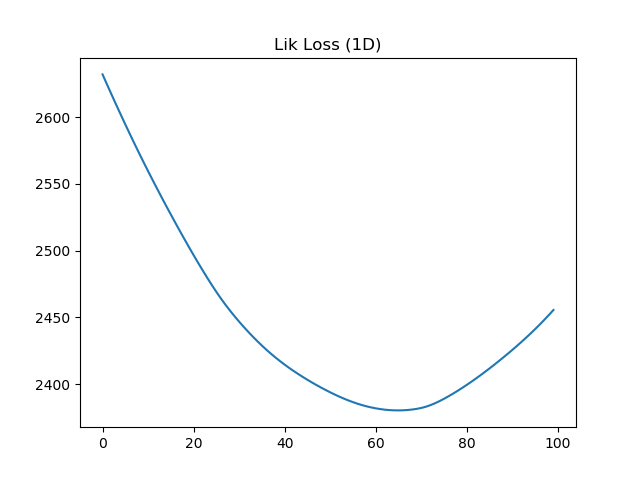
\includegraphics[width=7.5cm]{ex_1_6_fig_1.png}}}
    \qquad
    \subfloat{{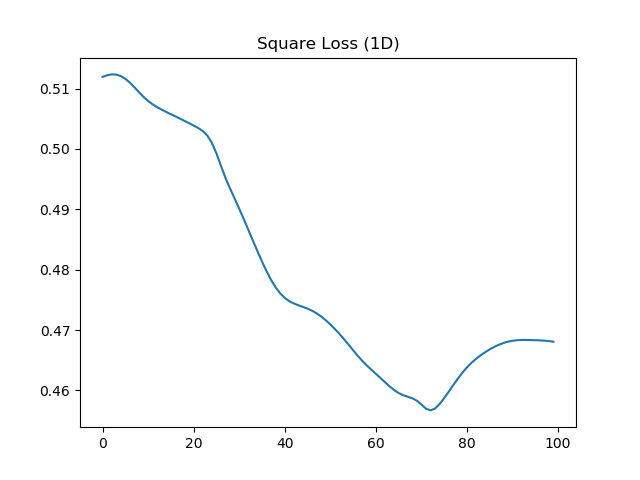
\includegraphics[width=7.5cm]{ex_1_6_fig_2.png}}}
    \caption{Slices of the 1-dimensional error surface of LikLoss and SquareLoss}
    \label{fig:ex16}
\end{figure}
\begin{figure}
    \centering
    \subfloat{{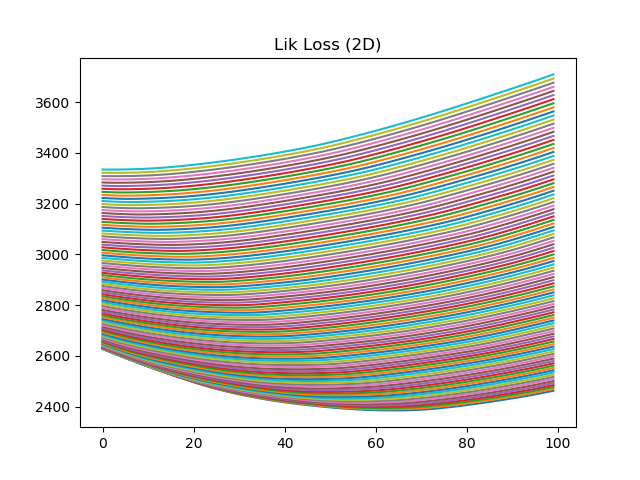
\includegraphics[width=7.5cm]{ex_1_7_fig_1.png}}}
    \qquad
    \subfloat{{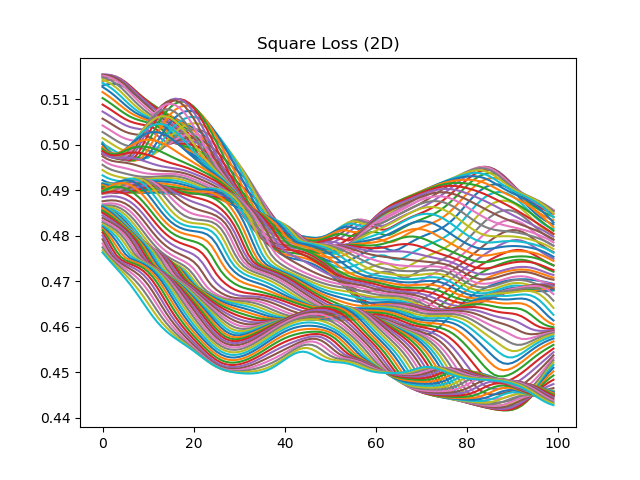
\includegraphics[width=7.5cm]{ex_1_7_fig_2.png}}}
    \caption{Slices of the 2-dimensional error surface of LikLoss and SquareLoss}
    \label{fig:ex17}
\end{figure}
For exercise 1.6, the supplied Julia code was used without any change, whereas in exercise 1.7 slight changes have been introduced to account for the additional dimension. The code below is the overall change to the given Julia to plot the four plots.
\begin{minted}{julia}
    # The values of the three coefficients are selected at random
    vec0=10*randn(D)
    vec1=10*randn(D)
    vec2=10*randn(D)
    
    # The number of steps in the [0, 1] interval to take
    I=100
    
    # The values for the two loss functions on 1 dimension
    Loss11=zeros(I);
    Loss12=zeros(I)
    
    # The values for the two loss functions on 2 dimensions
    Loss21=zeros(I,I);
    Loss22=zeros(I,I)
    
    for i=1:I
        # Compute the 1-dimensional error value for both losses
        lambda_i=i/I
        Loss11[i] = SquareLoss(c,NNpred(vec0+lambda_i*vec1,x))
        Loss12[i] = LikLoss(c,vec0+lambda_i*vec1,x)
        for j=1:I
            # Compute the 2-dimensional error value for both losses
            lambda_j=j/I
            Loss21[i,j] = SquareLoss(c,NNpred(vec0+lambda_i*vec1+lambda_j*vec2,x))
            Loss22[i,j] = LikLoss(c,vec0+lambda_i*vec1+lambda_j*vec2,x)
        end
    end
\end{minted}


\section*{Exercise 2}

\subsection*{Exercise 2.1}
The following loss function is given
\begin{equation}
    E = \sum_i \left( y_i - \sum_j W_{ij} x_j \right )^2
\end{equation}
\begin{figure}
    \centering
    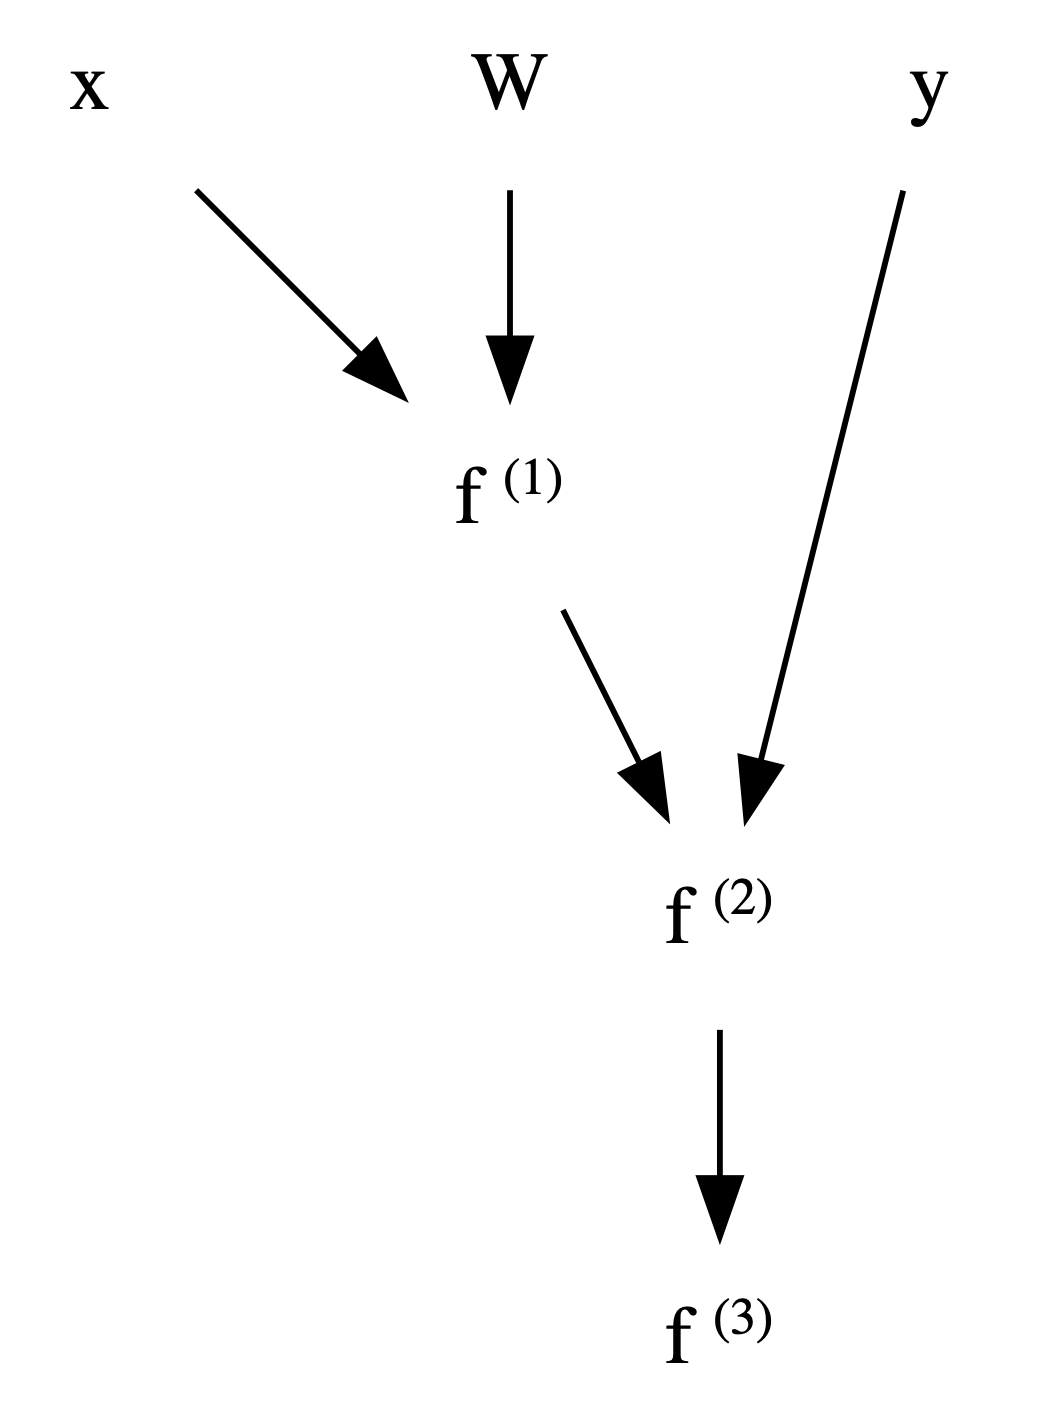
\includegraphics[height=2in]{cg21.png}
    \caption{The computation graph of the loss function in Exercise 2.1}
    \label{fig:cg21}
\end{figure}
and the exercise requires do compute the derivative
\begin{equation}
    \frac{\partial E}{\partial W_{ab}}
\end{equation}
The computation graph is drawn (figure \ref{fig:cg21}) and the functions are determined
\begin{equation}
    f^{(1)}_i = \sum_j W_{ij} x_j
\end{equation}
\begin{equation}
    f^{(2)}_i = y_i - f^{(1)}_i
\end{equation}
\begin{equation}
    f^{(3)} = \sum_i \left( f^{(2)}_i \right )^2
\end{equation}
The required partial derivatives are calculated.
\begin{equation}
    \begin{split}
        \frac{\partial f^{(1)}_i}{\partial W_{ab}} & =
        \frac{\partial}{\partial W_{ab}} \sum_j W_{ij} x_j \\
        & = \frac{\partial}{\partial W_{ab}} \left ( W_{i0} x_0 + W_{i1} x_1 + \dots + W_{ib} x_b + \dots + W_{in} x_n \right ) \\
        & = \delta_{ia} x_b
    \end{split}
\end{equation}
\begin{equation}
    \begin{split}
        \frac{\partial f^{(2)}_i}{\partial f^{(1)}_j} & =
        \frac{\partial}{\partial f^{(1)}_j}\left ( y_i - f^{(1)}_i \right )\\
        & = - \delta_{ij}
    \end{split}
\end{equation}
\begin{equation}
    \begin{split}
        \frac{\partial f^{(3)}}{\partial f^{(2)}_i} & =
        \frac{\partial}{\partial f^{(2)}_i} \sum_i \left( f^{(2)}_i \right )^2\\
        & = \frac{\partial}{\partial f^{(2)}_i}
        \left ( 2 f^{(2)}_0 + 2 f^{(2)}_1 + \dots + 2 f^{(2)}_i + \dots + 2 f^{(2)}_n  \right ) \\
        & = 2 f^{(2)}_i
    \end{split}
\end{equation}
The following reverse propagation schedules are defined.
\begin{equation}
    t^{(3)} = 1
\end{equation}
\begin{equation}
    t^{(2)}_i = \frac{\partial f^{(3)}}{\partial f^{(2)}_i} t^{(3)}
\end{equation}
\begin{equation}
    t^{(1)}_i = \sum_j \frac{\partial f^{(2)}_j}{\partial f^{(1)}_i} t^{(2)}_j
\end{equation}
\begin{equation}
    t^{W}_{ab} = \sum_i \frac{\partial f^{(1)}_i}{\partial W_{ab}} t^{(1)}_i
\end{equation}
From which the required derivative can be calculated.
\begin{equation}
    \begin{split}
        \frac{\partial E}{\partial W_{ab}} & = t^{W}_{ab} \\
        & = \sum_i \frac{\partial f^{(1)}_i}{\partial W_{ab}} t^{(1)}_i \\
        & = \sum_i \delta_{ia} x_b t^{(1)}_i \\
        & = x_b t^{(1)}_a \\
        & = x_b \sum_j \frac{\partial f^{(2)}_j}{\partial f^{(1)}_a} t^{(2)}_j \\
        & = x_b \sum_j - \delta_{ja} t^{(2)}_j \\
        & = - x_b t^{(2)}_a \\
        & = - x_b \frac{\partial f^{(3)}}{\partial f^{(2)}_a} t^{(3)} \\
        & = - 2 x_b f^{(2)}_a \\
        & = - 2 x_b \left ( y_a - f^{(1)}_a \right ) \\
        & = - 2 x_b \left ( y_a - \sum_i W_{ai} x_i \right )
    \end{split}
\end{equation}

\subsection*{Exercise 2.2}
An extended loss function (compared to the previous exercise) is given.
\begin{equation}
    E = \sum_i \left( y_i - \phi \left ( \sum_j W_{ij} x_j \right ) \right)^2
\end{equation}
\begin{figure}
    \centering
    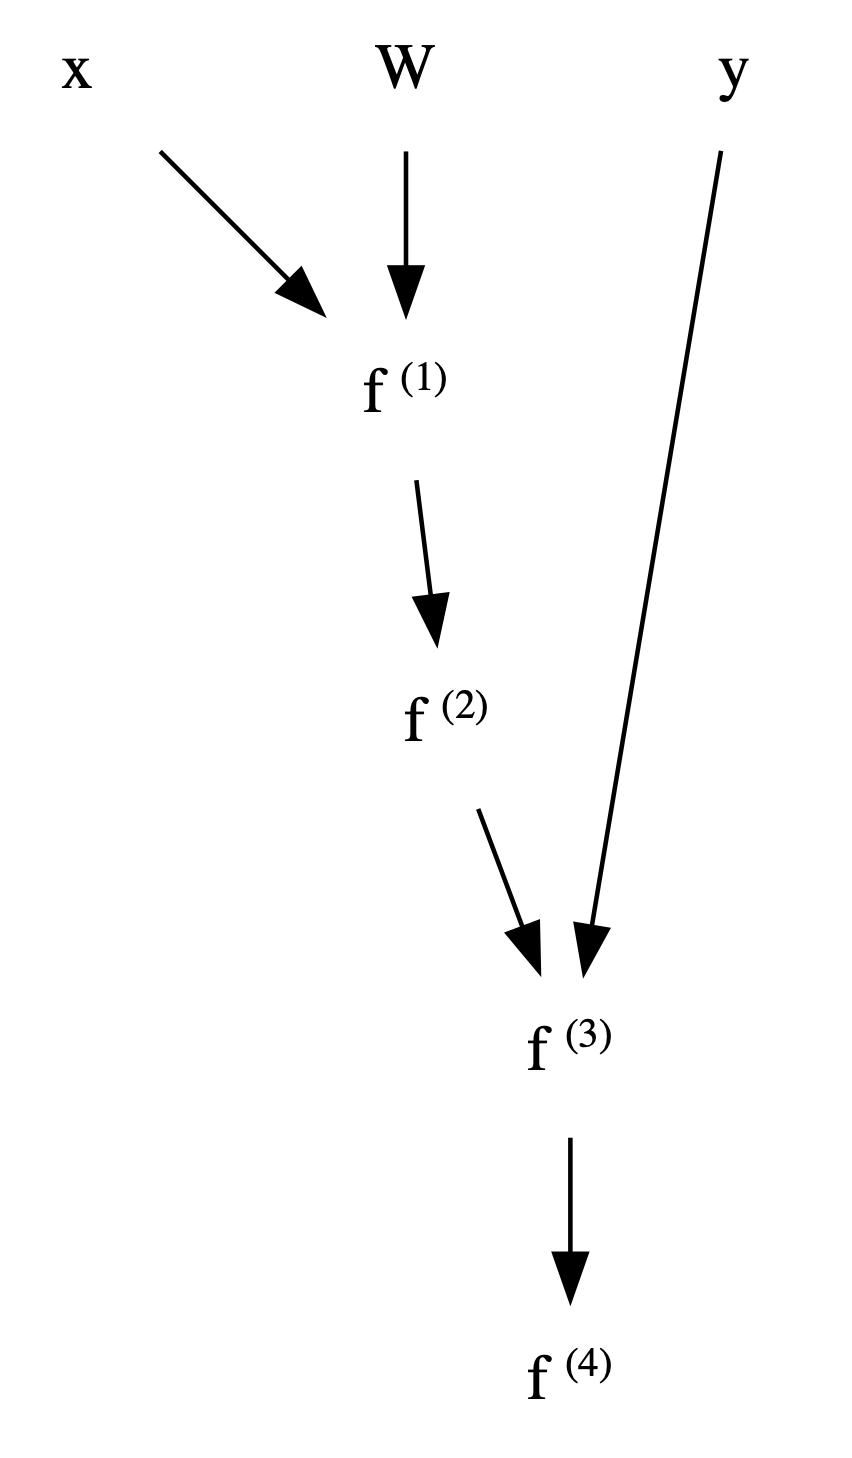
\includegraphics[height=2.5in]{cg22.png}
    \caption{The computation graph of the loss function in Exercise 2.2}
    \label{fig:cg22}
\end{figure}
and the exercise requires do compute the derivative
\begin{equation}
    \frac{\partial E}{\partial W_{ab}}
\end{equation}
The computation graph is drawn (figure \ref{fig:cg22}) the functions are derived
\begin{equation}
    f^{(1)}_i = \sum_j W_{ij} x_j
\end{equation}
\begin{equation}
    f^{(2)}_i = \phi (f^{(1)}_i)
\end{equation}
\begin{equation}
    f^{(3)}_i = y_i - f^{(2)}_i
\end{equation}
\begin{equation}
    f^{(4)} = \sum_i \left( f^{(2)}_i \right )^2
\end{equation}
The required partial derivatives are calculated.
\begin{equation}
    \begin{split}
        \frac{\partial f^{(1)}_i}{\partial W_{ab}} = \delta_{ia} x_b
    \end{split}
\end{equation}
\begin{equation}
    \begin{split}
        \frac{\partial f^{(2)}_i}{\partial f^{(1)}_j} = \phi'(f^{(1)}_j) \delta_{ij}
    \end{split}
\end{equation}
\begin{equation}
    \begin{split}
        \frac{\partial f^{(3)}_i}{\partial f^{(2)}_j} = - \delta_{ij}
    \end{split}
\end{equation}
\begin{equation}
    \begin{split}
        \frac{\partial f^{(4)}}{\partial f^{(3)}_i} = 2 f^{(3)}_i
    \end{split}
\end{equation}
The following reverse propagation schedules are defined.
\begin{equation}
    t^{(4)} = 1
\end{equation}
\begin{equation}
    t^{(3)}_i = \frac{\partial f^{(4)}}{\partial f^{(3)}_i} t^{(4)}
\end{equation}
\begin{equation}
    t^{(2)}_i = \sum_j \frac{\partial f^{(3)}_j}{\partial f^{(2)}_i} t^{(3)}_j
\end{equation}
\begin{equation}
    t^{(1)}_i = \sum_j \frac{\partial f^{(2)}_j}{\partial f^{(1)}_i} t^{(2)}_j
\end{equation}
\begin{equation}
    t^{W}_{ab} = \sum_i \frac{\partial f^{(1)}_i}{\partial W_{ab}} t^{(1)}_i
\end{equation}
From which the required derivative can be calculated.
\begin{equation}
    \begin{split}
        \frac{\partial E}{\partial W_{ab}} & = t^{W}_{ab} \\
        & = \sum_i \frac{\partial f^{(1)}_i}{\partial W_{ab}} t^{(1)}_i \\
        & = \sum_i \delta_{ia} x_b t^{(1)}_i \\
        & = x_b t^{(1)}_a \\
        & = x_b \sum_j \frac{\partial f^{(2)}_j}{\partial f^{(1)}_a} t^{(2)}_j \\
        & = x_b \sum_j \phi'(f^{(1)}_j) \delta_{aj} t^{(2)}_j \\
        & = x_b \phi'(f^{(1)}_a) t^{(2)}_a \\
        & = x_b \phi'(f^{(1)}_a) \sum_j \frac{\partial f^{(3)}_j}{\partial f^{(2)}_a} t^{(3)}_j \\
        & = x_b \phi'(f^{(1)}_a) \sum_j - \delta_{ja} t^{(3)}_j \\
        & = - x_b \phi'(f^{(1)}_a) t^{(3)}_a \\
        & = - x_b \phi'(f^{(1)}_a) \frac{\partial f^{(4)}}{\partial f^{(3)}_a} t^{(4)} \\
        & = - 2 f^{(3)}_a x_b \phi'(f^{(1)}_a) \\
    \end{split}
\end{equation}
This result can be proved by differentiating traditionally by applying the chain rule.
\begin{equation}
    \begin{split}
        \frac{d E}{d W_{ab}} & = \sum_i \left ( 2 f^{(3)}_i \right ) \left ( -1 \right ) \left ( \phi'\left(f^{(1)}_i \right) \right ) \left ( x_b \delta_{ia}\right ) =
        -2 f^{(3)}_a \phi'\left(f^{(1)}_a\right) x_b
    \end{split}
\end{equation}

\subsection*{Exercise 2.3}
The following loss function is given.
\begin{equation}
    E=\sum_i \left ( y_i - \phi_2 \left ( \sum_k W^{(2)}_{ik} \phi_1 \left ( \sum_j W^{(1)}_{kj} x_j \right ) \right ) \right )^2
\end{equation}
\begin{figure}
    \centering
    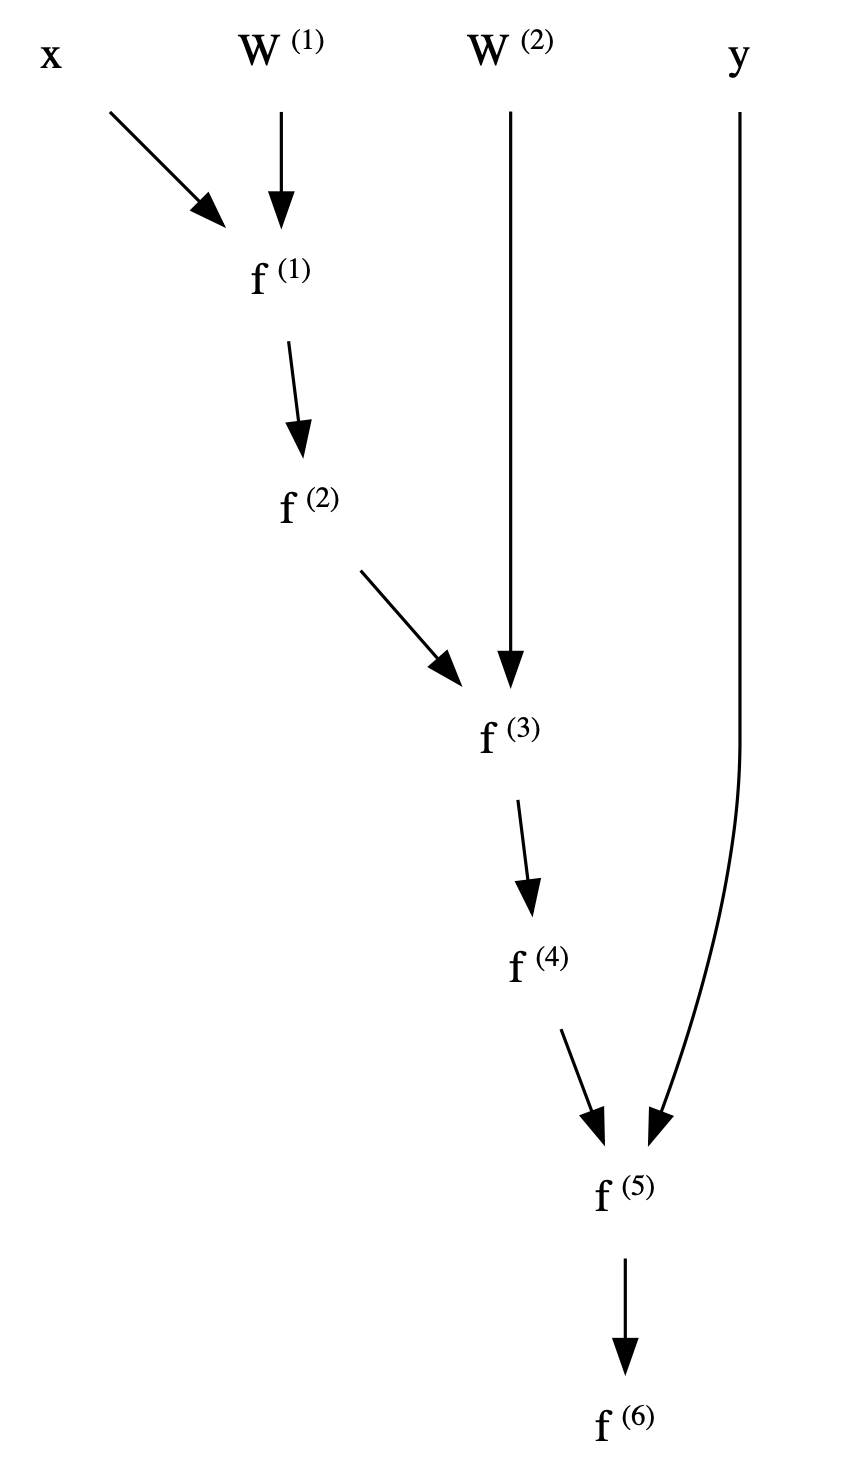
\includegraphics[height=3in]{cg23.png}
    \caption{The computation graph of the loss function in Exercise 2.3}
    \label{fig:cg23}
\end{figure}
The computation graph is drawn (figure \ref{fig:cg23}) The functions are defined.
\begin{equation}
    f^{(1)}_k = \sum_j W^{(1)}_{kj} x_j
\end{equation}
\begin{equation}
    f^{(2)}_k = \phi_1 (f^{(1)}_k)
\end{equation}
\begin{equation}
    f^{(3)}_i = \sum_k W^{(2)}_{ik} f^{(2)}_k
\end{equation}
\begin{equation}
    f^{(4)}_i = \phi_2 (f^{(3)}_i)
\end{equation}
\begin{equation}
    f^{(5)}_i = y_i - f^{(4)}_i
\end{equation}
\begin{equation}
    f^{(6)} = E = \sum_i \left ( f^{(5)}_i \right )^2
\end{equation}
The partial derivatives are calculated.
\begin{equation}
    \frac{\partial f^{(1)}_i}{\partial W^{(1)}_{ab}} = x_b \delta_{ia}
\end{equation}
\begin{equation}
    \frac{\partial f^{(2)}_i}{\partial f^{(1)}_j} = \phi'_1 \left ( f^{(1)}_i \right ) \delta_{ij}
\end{equation}
\begin{equation}
    \frac{\partial f^{(3)}_i}{\partial f^{(2)}_j} = W^{(2)}_{ij}
\end{equation}
\begin{equation}
    \frac{\partial f^{(3)}_i}{\partial W^{(2)}_{ab}} = f^{(2)}_b \delta_{ia}
\end{equation}
\begin{equation}
    \frac{\partial f^{(4)}_i}{\partial f^{(3)}_j} = \phi'_2 \left ( f^{(3)}_i \right ) \delta_{ij}
\end{equation}
\begin{equation}
    \frac{\partial f^{(5)}_i}{\partial f^{(4)}_j} = - \delta_{ij}
\end{equation}
\begin{equation}
    \frac{\partial f^{(6)}}{\partial f^{(5)}_i} = 2 f^{(5)}_i
\end{equation}
The propagation schedule is determined and messages calculated.
\begin{equation}
    t^{(6)} = 1
\end{equation}
\begin{equation}
    t^{(5)}_i = \frac{\partial f^{(6)}}{\partial f^{(5)}_i} t^{(6)} = 2 f^{(5)}_i t^{(6)}
\end{equation}
\begin{equation}
    t^{(4)}_i = \sum_j \frac{\partial f^{(5)}_j}{\partial f^{(4)}_i} t^{(5)}_j = \sum_j - \delta_{ji} t^{(5)}_j = - t^{(5)}_i
\end{equation}
\begin{equation}
    t^{(3)}_i = \sum_j \frac{\partial f^{(4)}_j}{\partial f^{(3)}_i} t^{(4)}_j = \sum_j \phi'_2 \left ( f^{(3)}_j \right ) \delta_{ji} t^{(4)}_j = \phi'_2 \left ( f^{(3)}_i \right ) t^{(4)}_i
\end{equation}
\begin{equation}
    t^{(2)}_i = \sum_j \frac{\partial f^{(3)}_j}{\partial f^{(2)}_i} t^{(3)}_j = \sum_j W^{(2)}_{ji} t^{(3)}_j
\end{equation}
\begin{equation}
    t^{(1)}_i = \sum_j \frac{\partial f^{(2)}_j}{\partial f^{(1)}_i} t^{(2)}_j = \sum_j \phi'_1 \left ( f^{(1)}_j \right ) \delta_{ji} t^{(2)}_j = \phi'_1 \left ( f^{(1)}_i \right ) t^{(2)}_i
\end{equation}
\begin{equation}
    t^{W^{(1)}}_{ab} = \sum_i \frac{\partial f^{(1)}_i}{\partial W^{(1)}_{ab}} t^{(1)}_i = \sum_i x_b \delta_{ia} t^{(1)}_i = x_b t^{(1)}_a
\end{equation}
\begin{equation}
    t^{W^{(2)}}_{ab} = \sum_i \frac{\partial f^{(3)}_i}{\partial W^{(2)}_{ab}} t^{(1)}_i = \sum_i f^{(2)}_b \delta_{ia} t^{(3)}_i = f^{(2)}_b t^{(3)}_a
\end{equation}
The required derivatives are calculated by joining messages.
\begin{equation}
    \begin{split}
        \frac{d E}{d W^{(1)}_{ab}} & = t^{W^{(1)}}_{ab} \\
        & = x_b t^{(1)}_a \\
        & = x_b \phi'_1 \left ( f^{(1)}_a \right ) t^{(2)}_a \\
        & = x_b \phi'_1 \left ( f^{(1)}_a \right ) \sum_j W^{(2)}_{ja} t^{(3)}_j \\
        & = x_b \phi'_1 \left ( f^{(1)}_a \right ) \sum_j W^{(2)}_{ja} \phi'_2 \left ( f^{(3)}_j \right ) t^{(4)}_j \\
        & = - x_b \phi'_1 \left ( f^{(1)}_a \right ) \sum_j W^{(2)}_{ja} \phi'_2 \left ( f^{(3)}_j \right ) t^{(5)}_j \\
        & = - 2 x_b \phi'_1 \left ( f^{(1)}_a \right ) \sum_j W^{(2)}_{ja} \phi'_2 \left ( f^{(3)}_j \right ) f^{(5)}_j
    \end{split}
\end{equation}
\begin{equation}
    \begin{split}
        \frac{d E}{d W^{(2)}_{ab}} & = t^{W^{(2)}}_{ab} \\
        & = f^{(2)}_b t^{(3)}_a \\
        & = f^{(2)}_b \phi'_2 \left ( f^{(3)}_a \right ) t^{(4)}_a \\
        & = - f^{(2)}_b \phi'_2 \left ( f^{(3)}_a \right ) t^{(5)}_a \\
        & = - 2 f^{(2)}_b \phi'_2 \left ( f^{(3)}_a \right ) f^{(5)}_a \\
    \end{split}
\end{equation}
These results are proved by differentiating in the traditional way with the chain rule.
\begin{equation}
    \begin{split}
        \frac{d E}{d W^{(1)}_{ab}} & =
        \sum_i \left ( 2 f^{(5)}_i \right ) \left ( -1 \right ) \left ( \phi'_2 \left ( f^{(3)}_i \right ) \right ) \sum_k W^{(2)}_{ik} \left ( \phi'_1 \left ( f^{(1)}_k \right ) \right ) \left ( x_b \delta_{ka} \right ) \\
        & = - 2 x_b \phi'_1 \left (f^{(1)}_a \right ) \sum_i f^{(5)}_i \phi'_2 \left ( f^{(3)}_i \right ) W^{(2)}_{ia}
    \end{split}
\end{equation}
\begin{equation}
    \begin{split}
        \frac{d E}{d W^{(2)}_{ab}} & =
        \sum_i \left ( 2 f^{(5)}_i \right ) \left ( -1 \right ) \left ( \phi'_2 \left ( f^{(3)}_i \right ) \right ) f^{(2)}_b \delta_{ia} \\
        & = - 2 f^{(5)}_a \phi'_2 \left ( f^{(3)}_a \right ) f^{(2)}_b
    \end{split}
\end{equation}

\subsection*{Exercise 2.4}
The loss functions observed in the previous exercises compute the loss for a given unit of data. This question, instead, requires to extend this scheme for all the units of data. In other words, rather than computing the loss for a single pair $(x, y)$, it requires to do so for the $n$ pairs $(x^n, y^n)$. Consequently, the loss function analysed in the previous exercise is extended by introducing a sum for each pair and the actual loss sees each occurrence $y$ and $x$ being replaced by $y^n$ and $x^n$, respectively. This is equivalent to computing the loss seen in the previous exercise for each unit of data and summing up the individual losses.
\begin{equation}
    E=\sum_n \sum_i \left ( y^n_i - \phi_2 \left ( \sum_k W^{(2)}_{ik} \phi_1 \left ( \sum_j W^{(1)}_{kj} x^n_j \right ) \right ) \right )^2
\end{equation}
Consequently, the individual functions are redefined to account for this change: all function previously defined will take an additional parameter $n$ which is passed down by the newly introduced function $f^{(7)} = E = \sum_n f^{(6)}_n$. Partial derivatives which are both passing down the unit index are updated accordingly, that is, a bind $\delta_{mn}$ is introduced for each derivative to ensure that within the summation for $n$ derivation is being carried out with respect to the same unit of data; the partial derivative $\frac{\partial f^{(7)}}{\partial f^{(6)}_{n}} = 1$ is added. The schedule is updated to reflect the introduction of the new parameter. Eventually, the two required derivatives are eventually calculated.
\begin{equation}
    \frac{d E}{d W^{(1)}_{ab}} =  - 2 \sum_n x^n_b \phi'_1 \left (f^{(1)}_{na} \right ) \sum_i f^{(5)}_{ni} \phi'_2 \left ( f^{(3)}_{ni} \right ) W^{(2)}_{ia}
\end{equation}
\begin{equation}
    \frac{d E}{d W^{(2)}_{ab}} = - 2 \sum_n f^{(5)}_{na} \phi'_2 \left ( f^{(3)}_{na} \right ) f^{(2)}_{nb}
\end{equation}

\subsection*{Exercise 2.5}
This exercise is similar to exercise 2.3 in that the two weights matrices are identical, such that $W^{(1)} = W^{(2)} = W$. Consequently, the loss function becomes
\begin{equation}
    E=\sum_i \left ( y_i - \phi_2 \left ( \sum_k W_{ik} \phi_1 \left ( \sum_j W_{kj} x_j \right ) \right ) \right )^2
\end{equation}
\begin{figure}
    \centering
    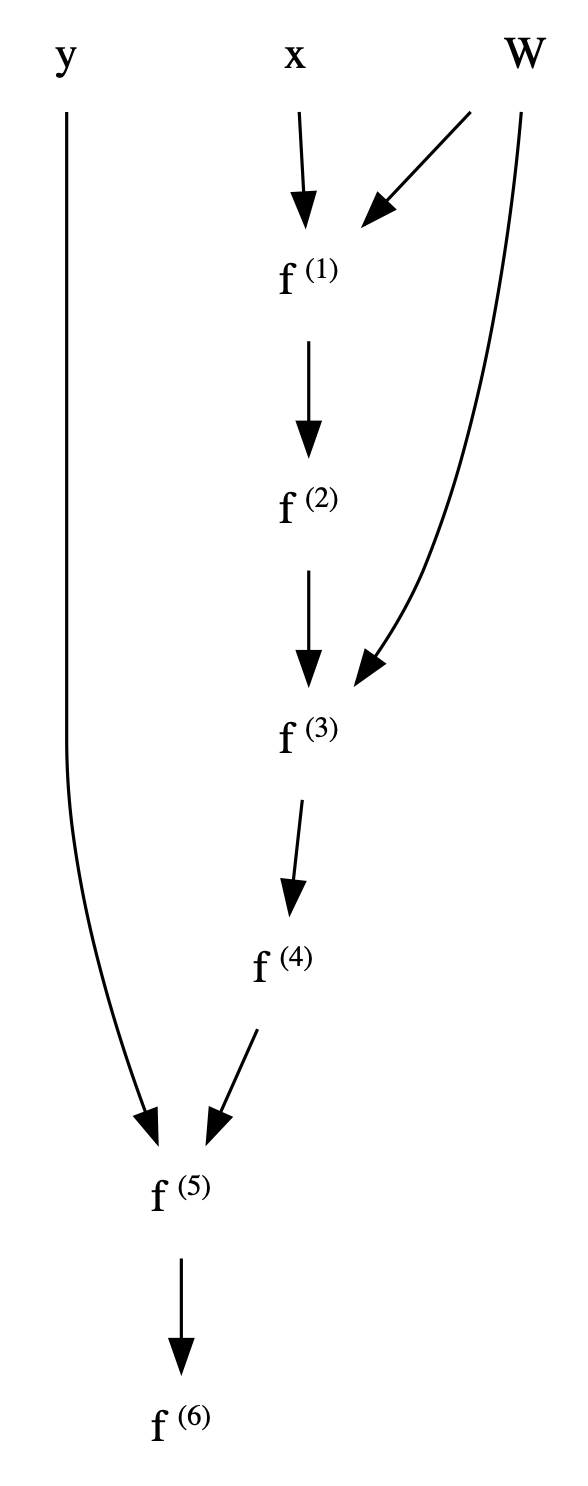
\includegraphics[height=3in]{cg25.png}
    \caption{The computation graph of the loss function in Exercise 2.5}
    \label{fig:cg25}
\end{figure}
The computation graph is drawn (figure \ref{fig:cg25}) the individual functions are updated.
\begin{equation}
    f^{(1)}_k = \sum_j W_{kj} x_j
\end{equation}
\begin{equation}
    f^{(2)}_k = \phi_1 (f^{(1)}_k)
\end{equation}
\begin{equation}
    f^{(3)}_i = \sum_k W_{ik} f^{(2)}_k
\end{equation}
\begin{equation}
    f^{(4)}_i = \phi_2 (f^{(3)}_i)
\end{equation}
\begin{equation}
    f^{(5)}_i = y_i - f^{(4)}_i
\end{equation}
\begin{equation}
    f^{(6)} = E = \sum_i \left ( f^{(5)}_i \right )^2
\end{equation}
Partial derivatives are updated as well.
\begin{equation}
    \frac{\partial f^{(1)}_i}{\partial W_{ab}} = x_b \delta_{ia}
\end{equation}
\begin{equation}
    \frac{\partial f^{(2)}_i}{\partial f^{(1)}_j} = \phi'_1 \left ( f^{(1)}_i \right ) \delta_{ij}
\end{equation}
\begin{equation}
    \frac{\partial f^{(3)}_i}{\partial f^{(2)}_j} = W_{ij}
\end{equation}
\begin{equation}
    \frac{\partial f^{(3)}_i}{\partial W_{ab}} = f^{(2)}_b \delta_{ia}
\end{equation}
\begin{equation}
    \frac{\partial f^{(4)}_i}{\partial f^{(3)}_j} = \phi'_2 \left ( f^{(3)}_i \right ) \delta_{ij}
\end{equation}
\begin{equation}
    \frac{\partial f^{(5)}_i}{\partial f^{(4)}_j} = - \delta_{ij}
\end{equation}
\begin{equation}
    \frac{\partial f^{(6)}}{\partial f^{(5)}_i} = 2 f^{(5)}_i
\end{equation}
Reverse schedules and messages are updated too.
\begin{equation}
    t^{(6)} = 1
\end{equation}
\begin{equation}
    t^{(5)}_i = \frac{\partial f^{(6)}}{\partial f^{(5)}_i} t^{(6)} = 2 f^{(5)}_i t^{(6)}
\end{equation}
\begin{equation}
    t^{(4)}_i = \sum_j \frac{\partial f^{(5)}_j}{\partial f^{(4)}_i} t^{(5)}_j = \sum_j - \delta_{ji} t^{(5)}_j = - t^{(5)}_i
\end{equation}
\begin{equation}
    t^{(3)}_i = \sum_j \frac{\partial f^{(4)}_j}{\partial f^{(3)}_i} t^{(4)}_j = \sum_j \phi'_2 \left ( f^{(3)}_j \right ) \delta_{ji} t^{(4)}_j = \phi'_2 \left ( f^{(3)}_i \right ) t^{(4)}_i
\end{equation}
\begin{equation}
    t^{(2)}_i = \sum_j \frac{\partial f^{(3)}_j}{\partial f^{(2)}_i} t^{(3)}_j = \sum_j W_{ji} t^{(3)}_j
\end{equation}
\begin{equation}
    t^{(1)}_i = \sum_j \frac{\partial f^{(2)}_j}{\partial f^{(1)}_i} t^{(2)}_j = \sum_j \phi'_1 \left ( f^{(1)}_j \right ) \delta_{ji} t^{(2)}_j = \phi'_1 \left ( f^{(1)}_i \right ) t^{(2)}_i
\end{equation}
\begin{equation}
    t^{W}_{ab} = \sum_i \frac{\partial f^{(1)}_i}{\partial W_{ab}} t^{(1)}_i + \sum_j \frac{\partial f^{(3)}_j}{\partial W_{ab}} t^{(3)}_j
\end{equation}
The main change is observed in $t^{W}_{ab}$ as it is updated to account for both \textit{paths}, as seen in the computation graph. The required derivative is then calculated with the new schedule.
\begin{equation}
    \begin{split}
        \frac{d E}{d W_{ab}} & = t^{W}_{ab} \\
        & = \sum_i \frac{\partial f^{(1)}_i}{\partial W_{ab}} t^{(1)}_i + \sum_k \frac{\partial f^{(3)}_k}{\partial W_{ab}} t^{(3)}_k \\
        & =
        \left( - 2 x_b \phi'_1 \left ( f^{(1)}_a \right ) \sum_j W^{(2)}_{ja} \phi'_2 \left ( f^{(3)}_j \right ) f^{(5)}_j \right) +
        \left( - 2 f^{(5)}_a \phi'_2 \left ( f^{(3)}_a \right ) f^{(2)}_b \right) \\
        & = -2 \left (f^{(5)}_a \phi'_2\left(f^{(3)}_a \right ) f^{(2)}_b + x_b \phi'_1 \left ( f^{(1)}_a \right ) \sum_j W^{(2)}_{ja} \phi'_2 \left ( f^{(3)}_j \right ) f^{(5)}_j \right )
    \end{split}
\end{equation}
This is confirmed by differentiating traditionally by applying the chain rule.
\begin{equation}
    \begin{split}
        \frac{d E}{d W_{ab}} & =
        \left ( \sum_i \left ( 2 f^{(5)}_i \right ) \left ( -1 \right ) \left ( \phi'_2 \left ( f^{(3)}_i \right ) \right ) \sum_k W_{ik} \left ( \phi'_1 \left ( f^{(1)}_k \right ) \right ) \left ( x_b \delta_{ka} \right ) \right ) + \\
        & + \left ( \sum_j \left ( 2 f^{(5)}_j \right ) \left ( -1 \right ) \left ( \phi'_2 \left ( f^{(3)}_j \right ) \right ) f^{(2)}_b \delta_{ia} \right ) \\
        & = - 2 f^{(5)}_a \phi'_2 \left ( f^{(3)}_a \right ) f^{(2)}_b - 2 x_b \phi'_1 \left (f^{(1)}_a \right ) \sum_i f^{(5)}_i \phi'_2 \left ( f^{(3)}_i \right ) W^{(2)}_{ia} \\
        & = - 2 \left ( f^{(5)}_a \phi'_2 \left ( f^{(3)}_a \right ) f^{(2)}_b + x_b \phi'_1 \left (f^{(1)}_a \right ) \sum_i f^{(5)}_i \phi'_2 \left ( f^{(3)}_i \right ) W^{(2)}_{ia} \right )
    \end{split}
\end{equation}

\section*{Exercise 3}
A neural network with a single hidden layer is given, representing an autoencoder for the $28 \times 28$ MNIST images.
\begin{equation}
    f_i(x) = \sigma \left (b^{(2)}_i + \sum_{k=1}^H W^{(2)}_{ik} \phi \left ( b^{(1)}_k + \sum_{j=1}^{784} W^{(1)}_{kj} x_j  \right ) \right )
\end{equation}
The error function $E$ is defined for a generic loss function $L$.
\begin{equation}
    E = \frac{1}{N} \sum_n^N \sum_i^{784} L\left(x^n_i, f_i\left(x^n\right)\right)
\end{equation}
\subsection*{Exercises 3.2 and 3.3}
The individual functions are defined and the related computation graph is drawn (figure \ref{fig:cg32}).
\begin{figure}
    \centering
    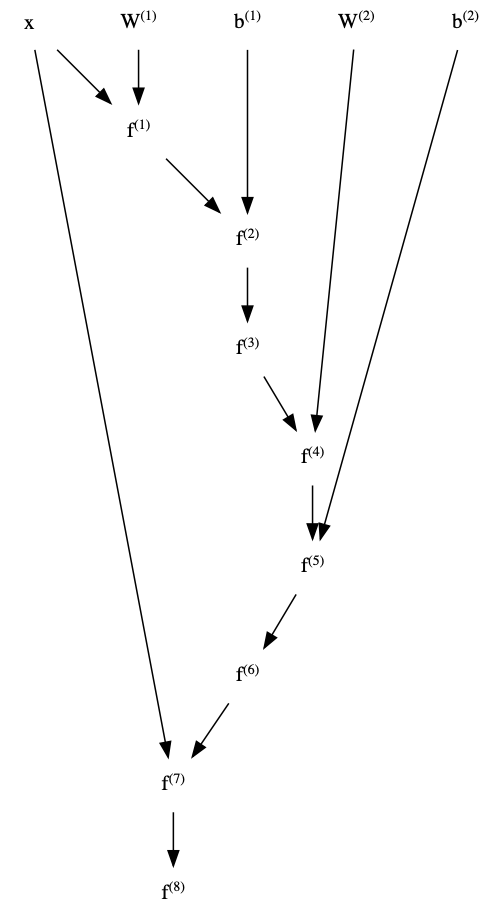
\includegraphics[height=3.5in]{cg32.png}
    \caption{The computation graph of the loss function in Exercise 3.2}
    \label{fig:cg32}
\end{figure}
\begin{equation}
    f^{(1)}_{nk} = \sum_{j=1}^{784} W^{(1)}_{kj} x^n_j
\end{equation}
\begin{equation}
    f^{(2)}_{nk} = b^{(1)}_k + f^{(1)}_{nk}
\end{equation}
\begin{equation}
    f^{(3)}_{nk} = \phi \left( f^{(2)}_{nk} \right )
\end{equation}
\begin{equation}
    f^{(4)}_{ni} = \sum_{k=1}^H W^{(2)}_{ik} f^{(3)}_{nk}
\end{equation}
\begin{equation}
    f^{(5)}_{ni} = b^{(2)}_i + f^{(4)}_{ni}
\end{equation}
\begin{equation}
    f^{(6)}_{ni} = \sigma \left ( f^{(5)}_{ni} \right )
\end{equation}
\begin{equation}
    f^{(7)}_{ni} = L\left(x_i^n, f^{(6)}_{ni}\right)
\end{equation}
\begin{equation}
    f^{(8)} = \frac{1}{N} \sum_n^N \sum_i^{784} f^{(7)}_{ni}
\end{equation}
The partial derivatives are calculated.
\begin{equation}
    \frac{\partial f^{(1)}_{ni}}{\partial W^{(1)}_{ab}} = \delta_{ia} x_b
\end{equation}
\begin{equation}
    \frac{\partial f^{(2)}_{ni}}{\partial f^{(1)}_{mj}} = \delta_{ij} \delta_{mn}
\end{equation}
\begin{equation}
    \frac{\partial f^{(2)}_{ni}}{\partial b^{(1)}_{a}} = \delta_{ia}
\end{equation}
\begin{equation}
    \frac{\partial f^{(3)}_{ni}}{\partial f^{(2)}_{mj}} = \phi'(f^{(2)}_{ni}) \delta_{ij} \delta_{mn}
\end{equation}
\begin{equation}
    \frac{\partial f^{(4)}_{ni}}{\partial f^{(3)}_{mj}} = W^{(2)}_{ij} \delta_{mn}
\end{equation}
\begin{equation}
    \frac{\partial f^{(4)}_{ni}}{\partial W^{(2)}_{ab}} = \delta_{ia} f^{(3)}_{nb}
\end{equation}
\begin{equation}
    \frac{\partial f^{(5)}_{ni}}{\partial f^{(4)}_{mj}} = \delta_{ij} \delta_{mn}
\end{equation}
\begin{equation}
    \frac{\partial f^{(5)}_{ni}}{\partial b^{(2)}_{a}} = \delta_{ia}
\end{equation}
\begin{equation}
    \frac{\partial f^{(6)}_{ni}}{\partial f^{(5)}_{mj}} = \sigma'\left(f^{(5)}_{ni}\right) \delta_{ij} \delta_{mn}
\end{equation}
\begin{equation}
    \frac{\partial f^{(7)}_{ni}}{\partial f^{(6)}_{mj}} = L'\left(x^n_i, f^{(6)}_{ni}\right) \delta_{ij} \delta_{mn}
\end{equation}
\begin{equation}
    \frac{\partial f^{(8)}}{\partial f^{(7)}_{ni}} = \frac{1}{N}
\end{equation}
The reverse schedule is determined along with the messages.
\begin{equation}
    t^{(8)} = 1
\end{equation}
\begin{equation}
    t^{(7)}_{ni} = \frac{\partial f^{(8)}}{\partial f^{(7)}_ni} t^{(8)} = \frac{1}{N} t^{(8)}
\end{equation}
\begin{equation}
    t^{(6)}_{ni} = \sum_m \sum_j \frac{\partial f^{(7)}_{mj}}{\partial f^{(6)}_ni} t^{(7)}_{mj} = \sum_m \sum_j L'\left(x^m_j, f^{(6)}_{mj}\right) \delta_{ij} \delta_{mn} t^{(7)}_{mj} = L'\left(x^n_i, f^{(6)}_{ni}\right) t^{(7)}_{ni}
\end{equation}
\begin{equation}
    t^{(5)}_{ni} = \sum_m \sum_j \frac{\partial f^{(6)}_{mj}}{\partial f^{(5)}_ni} t^{(6)}_{mj} = \sum_m \sum_j \sigma'\left(f^{(5)}_{mj}\right) \delta_{ij} \delta_{mn} t^{(6)}_{mj} = \sigma'\left(f^{(5)}_{ni}\right) t^{(6)}_{ni}
\end{equation}
\begin{equation}
    t^{b^{(2)}}_{a} = \sum_m \sum_j \frac{\partial f^{(5)}_{mj}}{\partial b^{(2)}_a} t^{(5)}_{mj} = \sum_m \sum_j \delta_{ja} t^{(5)}_{mj} = \sum_m t^{(5)}_{ma}
\end{equation}
\begin{equation}
    t^{(4)}_{ni} = \sum_m \sum_j \frac{\partial f^{(5)}_{mj}}{\partial f^{(4)}_ni} t^{(5)}_{mj} = \sum_m \sum_j \delta_{ij} \delta_{mn} t^{(5)}_{mj} = t^{(5)}_{ni}
\end{equation}
\begin{equation}
    t^{W^{(2)}}_{ab} = \sum_n \sum_i \frac{\partial f^{(4)}_{ni}}{\partial W^{(2)}_{ab}} t^{(4)}_{ni} = \sum_n \sum_i \delta_{ia} f^{(3)}_{nb} t^{(4)}_{ni} = \sum_n f^{(3)}_{nb} t^{(4)}_{na}
\end{equation}
\begin{equation}
    t^{(3)}_{ni} = \sum_m \sum_j \frac{\partial f^{(4)}_{mj}}{\partial f^{(3)}_ni} t^{(4)}_{mj} = \sum_m \sum_j W^{(2)}_{ji} \delta_{mn} t^{(4)}_{mj} = \sum_j W^{(2)}_{ji} t^{(4)}_{nj}
\end{equation}
\begin{equation}
    t^{(2)}_{ni} = \sum_m \sum_j \frac{\partial f^{(3)}_{mj}}{\partial f^{(2)}_ni} t^{(3)}_{mj} = \sum_m \sum_j \phi ' \left (f^{(2)}_{mj}\right) \delta_{ij} \delta_{mn} t^{(3)}_{mj} = \phi ' \left (f^{(2)}_{ni}\right) t^{(3)}_{ni}
\end{equation}
\begin{equation}
    t^{(1)}_{ni} = \sum_m \sum_j \frac{\partial f^{(2)}_{mj}}{\partial f^{(1)}_ni} t^{(2)}_{mj} = \sum_m \sum_j \delta_{ij} \delta_{mn} t^{(2)}_{mj} = t^{(2)}_{ni}
\end{equation}
\begin{equation}
    t^{b^{(1)}}_{a} = \sum_m \sum_j \frac{\partial f^{(2)}_{mj}}{\partial b^{(1)}_a} t^{(2)}_{mj} = \sum_m \sum_j \delta_{ja} t^{(2)}_{mj} = \sum_m t^{(2)}_{ma}
\end{equation}
\begin{equation}
    t^{W^{(1)}}_{ab} = \sum_m \sum_j \frac{\partial f^{(1)}_{mj}}{\partial W^{(1)}_{ab}} t^{(1)}_{mj} = \sum_m \sum_j x_b \delta_{ja} t^{(2)}_{mj} =
    \sum_m x_b t^{(1)}_{ma}
\end{equation}
The required derivatives are then computed using the schedule and messages.
\begin{equation}
    \begin{split}
        \frac{d E}{d W^{(1)}_{ab}} & = t^{W^{(1)}}_{ab} \\
        & = \sum_n x_b t^{(1)}_{na} \\
        & = \sum_n x_b t^{(2)}_{na} \\
        & = \sum_n x_b \phi ' \left (f^{(2)}_{na}\right) t^{(3)}_{na} \\
        & = \sum_n x_b \phi ' \left (f^{(2)}_{na}\right) \sum_i W^{(2)}_{ia} t^{(4)}_{ni} \\
        & = \sum_n x_b \phi ' \left (f^{(2)}_{na}\right) \sum_i W^{(2)}_{ia} t^{(5)}_{ni} \\
        & = \sum_n x_b \phi ' \left (f^{(2)}_{na}\right) \sum_i W^{(2)}_{ia} \sigma'\left(f^{(5)}_{ni}\right) t^{(6)}_{ni} \\
        & = \sum_n x_b \phi ' \left (f^{(2)}_{na}\right) \sum_i W^{(2)}_{ia} \sigma'\left(f^{(5)}_{ni}\right) L'\left(x^n_i, f^{(6)}_{ni}\right) t^{(7)}_{ni} \\
        & = \frac{1}{N} \sum_n x_b \phi ' \left (f^{(2)}_{na}\right) \sum_i W^{(2)}_{ia} \sigma'\left(f^{(5)}_{ni}\right) L'\left(x^n_i, f^{(6)}_{ni}\right) \\
    \end{split}
\end{equation}
\begin{equation}
    \begin{split}
        \frac{d E}{d b^{(1)}_{a}} & = t^{b^{(1)}}_{a} \\
        & = \sum_n t^{(2)}_{na} \\
        & = \sum_n \phi ' \left (f^{(2)}_{na}\right) t^{(3)}_{na} \\
        & = \sum_n \phi ' \left (f^{(2)}_{na}\right) \sum_i W^{(2)}_{ia} t^{(4)}_{ni} \\
        & = \sum_n \phi ' \left (f^{(2)}_{na}\right) \sum_i W^{(2)}_{ia} t^{(5)}_{ni} \\
        & = \sum_n \phi ' \left (f^{(2)}_{na}\right) \sum_i W^{(2)}_{ia} \sigma'\left(f^{(5)}_{ni}\right) L'\left(x^n_i, f^{(6)}_{ni}\right) t^{(7)}_{ni} \\
        & = \frac{1}{N} \sum_n \phi ' \left (f^{(2)}_{na}\right) \sum_i W^{(2)}_{ia} \sigma'\left(f^{(5)}_{ni}\right) L'\left(x^n_i, f^{(6)}_{ni}\right) \\
    \end{split}
\end{equation}
\begin{equation}
    \begin{split}
        \frac{d E}{d W^{(2)}_{ab}} & = t^{W^{(2)}}_{ab} \\
        & = \sum_n f^{(3)}_{nb} t^{(4)}_{na} \\
        & = \sum_n f^{(3)}_{nb} t^{(5)}_{na} \\
        & = \sum_n f^{(3)}_{nb} \sigma'\left(f^{(5)}_{na}\right) t^{(6)}_{na} \\
        & = \sum_n f^{(3)}_{nb} \sigma'\left(f^{(5)}_{na}\right) L'\left(x^n_a, f^{(6)}_{na}\right) t^{(7)}_{na} \\
        & = \frac{1}{N} \sum_n f^{(3)}_{nb} \sigma'\left(f^{(5)}_{na}\right) L'\left(x^n_a, f^{(6)}_{na}\right)
    \end{split}
\end{equation}
\begin{equation}
    \begin{split}
        \frac{d E}{d b^{(2)}_{a}} & = t^{b^{(2)}}_{a} \\
        & = \sum_n t^{(5)}_{na} \\
        & = \sum_n \sigma'\left(f^{(5)}_{na}\right) t^{(6)}_{na} \\
        & = \sum_n \sigma'\left(f^{(5)}_{na}\right) L'\left(x^n_a, f^{(6)}_{na}\right) t^{(7)}_{na} \\
        & = \frac{1}{N} \sum_n \sigma'\left(f^{(5)}_{na}\right) L'\left(x^n_a, f^{(6)}_{na}\right)
    \end{split}
\end{equation}
\subsection*{Exercise 3.4 and 3.5}
For this question, Python was used to implement the ADAM optimiser, along with the previously defined AutoDiff schedule. Different transfer functions were tested and the relu was chosen; initial weights are picked randomly from a zero-mean unit-variance normal distribution. Learning rate was set to $0.05$, while the three ADAM parameters were tuned as suggested. The error decrease can be observed in figure \ref{fig:loss}; results of reconstruction with the autoencoder can be observed in figure \ref{fig:mnist1}.
\begin{figure}[H]
    \centering
    \subfloat{{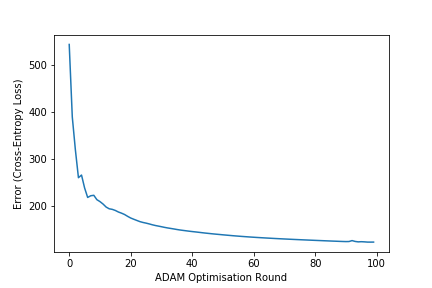
\includegraphics[width=7.5cm]{training_error_cross.png}}}
    \qquad
    \subfloat{{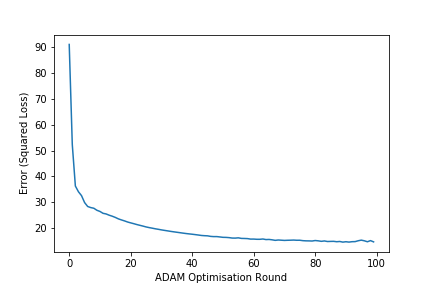
\includegraphics[width=7.5cm]{training_error_squared.png}}}
    \caption{Training error at each ADAM optimisation round with Square Loss (left) and Cross Entropy Loss (right).}
    \label{fig:loss}
\end{figure}
\begin{figure}
    \centering
    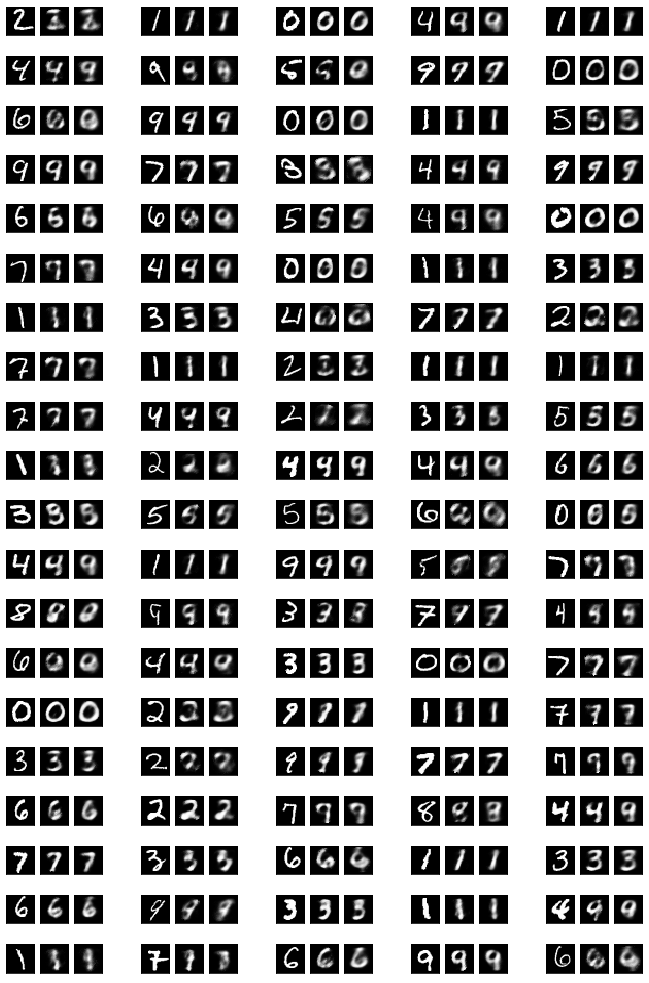
\includegraphics[width=5.5in]{whole_plot.png}
    \caption{The reconstructions of 100 MNIST digits; each triplet contains (from left to right) the original image, the reconstruction using squared loss and cross-entropy loss.}
    \label{fig:mnist1}
\end{figure}

\subsection*{Exercise 3.6}
This question requires to determine whether the error function is convex with respect to $W^2$ and $b^2$ for both the LikLoss and SquareLoss. As usual, convexity is determined by whether the second derivative is always positive. For convenience, throughout this exercise, $\sigma$ is used to represent $f^{(6)}_{na} = \sigma \left ( f^{(5)}_{na} \right )$ and $L$ to represent $L \left(x^n_a, f^{(6)}_{na}\right)$; the single apex $'$ and double apex $''$ represent the first and second derivative of the function they follow with respect to either of the two variables of interest. The loss functions and their derivatives with respect to the second parameter $y$ (which will be the one of interest in the calculations) are
\begin{equation}
    L_{lik}(x, y) = - x \log ( y ) - (1-x)\log(1-y)
\end{equation}
\begin{equation}
    L'_{lik}(x, y) = \frac{y-x}{y(1-y)}
\end{equation}
\begin{equation}
    L''_{lik}(x, y) = \frac{y^2+x-2xy}{y^2(1-y)^2}
\end{equation}
\begin{equation}
    L_{sq}(x, y) = \frac{1}{2} (x -  y)^2
\end{equation}
\begin{equation}
    L'_{sq}(x, y) = y - x
\end{equation}
\begin{equation}
    L''_{sq}(x, y) = 1
\end{equation}
With regard to $b^{(2)}$, the first and second derivatives are:
\begin{equation}
    \frac{\partial E}{\partial b^{(2)}_{a}} = \frac{1}{N} \sum_n \sigma'\left(f^{(5)}_{na}\right) L'\left(x^n_a, f^{(6)}_{na}\right) = \frac{1}{N} \sum_n \sigma' L'
\end{equation}
\begin{equation}
    \begin{split}
        \frac{\partial^2 E}{\partial {b^{(2)}_{a}}^2} & =
        \frac{1}{N} \sum_n \sigma'L''\sigma' + \sigma''L' \\
        & = \frac{1}{N} \sum_n \sigma^2 (1-\sigma)^2 L'' + \sigma (1-\sigma)(1-2\sigma) L' \\
        & = \frac{1}{N} \sum_n \sigma (1-\sigma)[\sigma(1-\sigma)L'' + (1-2\sigma)L']
    \end{split}
\end{equation}
It is known that $\sigma (1-\sigma)$ is never negative, hence the factor to assess for positivity is $\sigma(1-\sigma)L'' + (1-2\sigma)L'$. For the LikLoss:
\begin{equation}
    \sigma(1-\sigma)\frac{\sigma^2 + x -2\sigma x}{\sigma^2 (1-\sigma)^2} + (1-2\sigma)\frac{\sigma -x}{\sigma(1-\sigma)} = \frac{x + \sigma^2 -2\sigma x + \sigma -x -2\sigma^2 +2\sigma x}{\sigma(1-\sigma)} = 1
\end{equation}
This proves that the second derivative of the error function with respect to $b^{(2)}$ using the LikLoss is always positive, proving convexity. Similarly, for the SquareLoss:
\begin{equation}
        \sigma(1-\sigma) +(1-2\sigma)(\sigma-x) = \sigma - \sigma^2 + \sigma - x - 2\sigma^2 + 2\sigma x = -3\sigma^2 + \sigma(2+2x) - x
\end{equation}
For the error function to be convex, this factor has to be positive for each value of $x$, but that is not the case as the function can be negative (e.g. for $\sigma=0.75, x = 0$ the factor is equal to $-0.1875$). Due to this inconsistency in the sign of the factor, it is determined that the error function is not convex with respect to $b^{(2)}$ when the SquareLoss is used.\\ \ \\
The process is now repeated for $W^{(2)}$. The derivative of the error function with respect to $W^{(2)}_{ab}$ is:
\begin{equation}
    \frac{\partial E}{\partial W^{(2)}_{ab}} = \frac{1}{N} \sum_n f^{(3)}_{nb} \sigma'\left(f^{(5)}_{na}\right) L'\left(x^n_a, f^{(6)}_{na}\right)
\end{equation}
The factor $f^{(3)}$ does not depend on $W^{(2)}$ and can therefore be treated as a constant. The second derivative is:
\begin{equation}
    \begin{split}
        \frac{\partial ^2 E}{\partial {W^{(2)}_{ab}}^2} & = \frac{1}{N} \sum_n f^{(3)}_{nb} \left [
        \sigma'\left(f^{(5)}_{na}\right) L''\left(x^n_a, f^{(6)}_{na}\right) \sigma'\left(f^{(5)}_{na}\right) f^{(3)}_{nb} + L'\left(x^n_a, f^{(6)}_{na}\right) \sigma''\left(f^{(5)}_{na}\right) f^{(3)}_{nb}
        \right] \\
        & = \frac{1}{N} \sum_n \left(f^{(3)}_{nb}\right)^2 \left [
        \left(\sigma'\left(f^{(5)}_{na}\right)\right)^2 L''\left(x^n_a, f^{(6)}_{na}\right) + L'\left(x^n_a, f^{(6)}_{na}\right) \sigma''\left(f^{(5)}_{na}\right)
        \right] \\
        & = \frac{1}{N} \sum_n \left(f^{(3)}_{nb}\right)^2 \left[
        (\sigma ')^2 L'' + \sigma'' L' \right] \\
        & = \frac{1}{N} \sum_n \left(f^{(3)}_{nb}\right)^2 \left[
        \sigma^2 (1-\sigma)^2 L'' + \sigma (1-\sigma)(1-2 \sigma) L' \right] \\
        & = \frac{1}{N} \sum_n \left(f^{(3)}_{nb}\right)^2 \sigma (1-\sigma) \left[
        \sigma (1-\sigma) L'' + \sigma (1-2 \sigma) L' \right]
    \end{split}
\end{equation}
The only factor to assess is once again $\sigma (1-\sigma) L'' + \sigma (1-2 \sigma) L'$. The conclusions on its sign are similar to the ones in the first half of this exercise. This means that for the LikLoss, the error function is concave with respect to $W^{(2)}$, but it is not for the SquareLoss.

\subsection*{Exercise 3.7 and 3.8}
In these questions, slices of the error function with the Square Loss first and Cross-Entropy Loss then are plotted to observe whether they are convex or not. In particular, the functions plotted are
\begin{equation}
    F_{11}(z_1, z_2) = E(W^{(1)} + z_1 U^{(1)} + z_2 ^{(2)} U^{(2)}, b^{(1)}, W^{(2)}, b^{(2)})
\end{equation}
\begin{equation}
    F_{12}(z_1, z_2) = E(W^{(1)} + z_1 U^{(1)}, b^{(1)}, W^{(2)} + z_2 U^{(2)}, b^{(2)})
\end{equation}
\begin{equation}
    F_{22}(z_1, z_2) = E(W^{(1)}, b^{(1)}, W^{(2)} + z_1 U^{(1)} + z_2 ^{(2)} U^{(2)}, b^{(2)})
\end{equation}
for both loss functions, results are in figures \ref{fig:error_plot_1}, \ref{fig:error_plot_2} and \ref{fig:error_plot_3}. It can be observed that with cross-entropy loss, the error function appears to be convex, whereas with square loss, the error function is not convex.
\begin{figure}[H]
    \centering
    \subfloat{{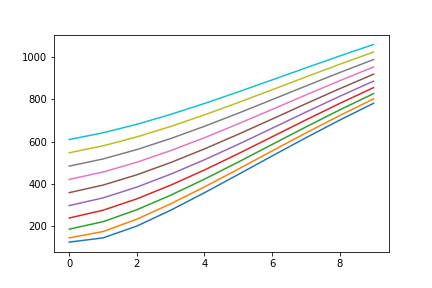
\includegraphics[width=7.5cm]{error_plot_1_cross.png}}}
    \qquad
    \subfloat{{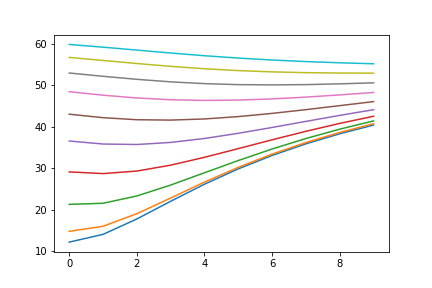
\includegraphics[width=7.5cm]{error_plot_1_square.png}}}
    \caption{$F_{1,1}$ for Cross-Entropy Loss (left) and Square Loss (Right)}
    \label{fig:error_plot_1}
\end{figure}
\begin{figure}[H]
    \centering
    \subfloat{{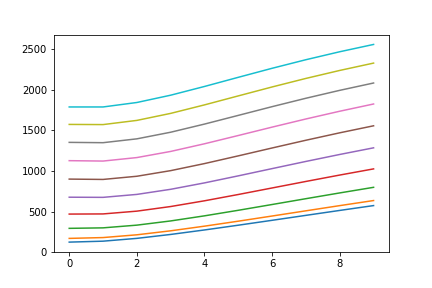
\includegraphics[width=7.5cm]{error_plot_2_cross.png}}}
    \qquad
    \subfloat{{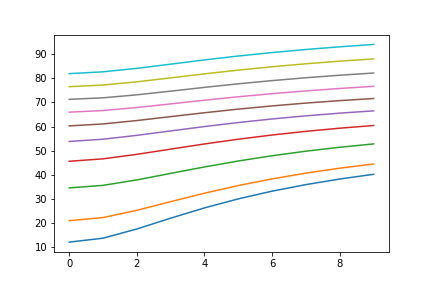
\includegraphics[width=7.5cm]{error_plot_2_square.png}}}
    \caption{$F_{1,2}$ for Cross-Entropy Loss (left) and Square Loss (Right)}
    \label{fig:error_plot_2}
\end{figure}
\begin{figure}[H]
    \centering
    \subfloat{{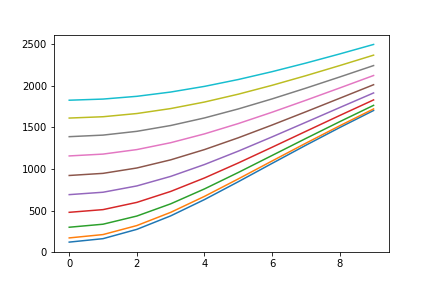
\includegraphics[width=7.5cm]{error_plot_3_cross.png}}}
    \qquad
    \subfloat{{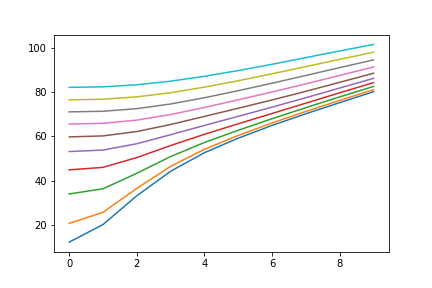
\includegraphics[width=7.5cm]{error_plot_3_square.png}}}
    \caption{$F_{2,2}$ for Cross-Entropy Loss (left) and Square Loss (Right)}
    \label{fig:error_plot_3}
\end{figure}

\section*{Code}

\subsection*{MNIST Autoencoder}
The following code was used in Question 3.
\begin{minted}{python}
def sigmoid(x):
    return 1 / (1 + np.exp(0 - x))
    
def relu(x):
    return np.maximum(x,0)

def d_relu(x):
    return np.where(x > 0, np.full(np.shape(x), 1), np.full(np.shape(x), 0))

def squared_loss(y, x):
    return (y - x) ** 2 / 2

def d_squared_loss(y, x):
    return - (y - x)

def cross_entropy_loss(x,y):
    return -x*np.log(y) - (1-x)*np.log(1-y)

def d_cross_entropy_loss(x,y):
    return ((1-x)/(1-y)) - (x/y)
    
def create_weight(shape):
    stdv = 1. / np.sqrt(shape[-1])
    return np.random.uniform(-stdv, stdv, shape).astype(np.float32)

def autodiff(xs, w1, w2, b1, b2):
    """ Performs automatic differntiation for the required network.
    
    :param xs: the matrix of features
    :param w1, w2, b1, b2: the matrices and vectors for the pairs of weights and biases
    :return: the matrix representing the loss for each value in xs, the matrices
    representing the total derivative of the error function for each value
    in xs for w1, w2, b1 and b2, the matrix representing the error for each value in xs """
    N = xs.shape[1]
    D = xs.shape[0]
    f1 = w_1 @ xs
    f2 = (b_1 + f1.T).T
    f3 = relu(f2)
    f4 = w_2 @ f3
    f5 = (b_2 + f4.T).T
    f6 = sigmoid(f5)
    f7 = loss(xs, f6)
    f8 = np.sum(f7, axis=0)
    f9 = np.sum(f8)
    f10 = f9 / N
    t10 = 1
    t9 = 1 / N
    t8 = np.full((N), 1 / N)
    t7 = np.full((D, N), 1 / N)
    t6 = d_loss(xs, f6) * t7
    t5 = (f6*(1-f6)) * t6
    t4 = t5
    tb2 = np.sum(t5, axis=1)
    t3 = w_2.T @ t4
    tw2 = (f3 @ t4.T).T
    t2 = d_relu(f2) * t3
    t1 = t2
    tb1 = np.sum(t2, axis=1)
    tw1 = t1 @ xs.T
    return f6, tw1, tw2, tb1, tb2, f10
    
def adam(weight, grad, k, m_prev, v_prev, b1=0.9, b2=0.999, l=0.0000000001, rate=0.05):
    """ Performs ADAM optimisaton.
    
    :param weight: the list of weights to optimise
    :param grad: the gradient for the error function at the weights
    :param k: the round of optimisation
    :param m_prev, v_prev: the ADAM parameters at the previous round
    :return: the next round of optimisation, the ADAM parameters for the round """
    m = b1 * m_prev + (1 - b1)*grad
    v = b2 * v_prev + (1 - b2)*(grad ** 2)
    m_hat = m / (1 - (b1 ** k))
    v_hat = v / (1 - (b2 ** k))
    weight -= (rate / (np.sqrt(v_hat) + l))*m_hat
    return (k+1, m, v)
    
w1 = create_weight((30, 784))
w2 = create_weight((784, 30))
b1 = create_weight((30,))
b2 = create_weight((784,))

epochs = 100

past_epochs = []
past_loss_values = []

previous_runnings = [[1,0,0] for i in range(4)]
weights = [w1,w2,b1,b2]

for i in range(epochs):
    res, grad_w1, grad_w2, grad_b1, grad_b2, loss = run(features.T, w1, w2, b1, b2)
    grads = [grad_w1, grad_w2, grad_b1, grad_b2]
    for (j, (weight, previous_running, grad)) in enumerate(zip(weights, previous_runnings, grads)):
        k, m, v = previous_running
        previous_runnings[j] = adam(weight, grad, k, m, v)
    past_epochs.append(i)
    past_loss_values.append(loss)

\end{minted}





































\end{document}
